\documentclass[a4paper,12pt]{report} % добавить leqno в [] для нумерации слева

%%% Работа с русским языком
\usepackage{cmap}					% поиск в PDF
\usepackage{mathtext} 				% русские буквы в формулах
\usepackage[T2A]{fontenc}			% кодировка
\usepackage[utf8]{inputenc}			% кодировка исходного текста
\usepackage[english,russian]{babel}	% локализация и переносы

\usepackage{graphicx}				%вставка изображений(графиков, в частности)
\usepackage{alltt}

%%% Дополнительная работа с математикой
\usepackage{amsmath,amsfonts,amssymb,amsthm,mathtools} % AMS
\usepackage{icomma} % "Умная" запятая: $0,2$ --- число, $0, 2$ --- перечисление

%% Номера формул
\mathtoolsset{showonlyrefs=true} % Показывать номера только у тех формул, на которые есть \eqref{} в тексте.

%% Шрифты
\usepackage{euscript}	 % Шрифт Евклид
\usepackage{mathrsfs} % Красивый матшрифт

%% Свои команды
\DeclareMathOperator{\sgn}{\mathop{sgn}}

%\setlength\parindent{0ex}
%\setlength\parskip{0.3cm}

%\renewcommand{\arraystretch}{1.8}

%%% Заголовок
\author{Волков Павел А-14-19}
\title{Отчет по Лабораторной работе №2}
\date{\today}

\begin{document}

Вот график окрестностей корней

\noindent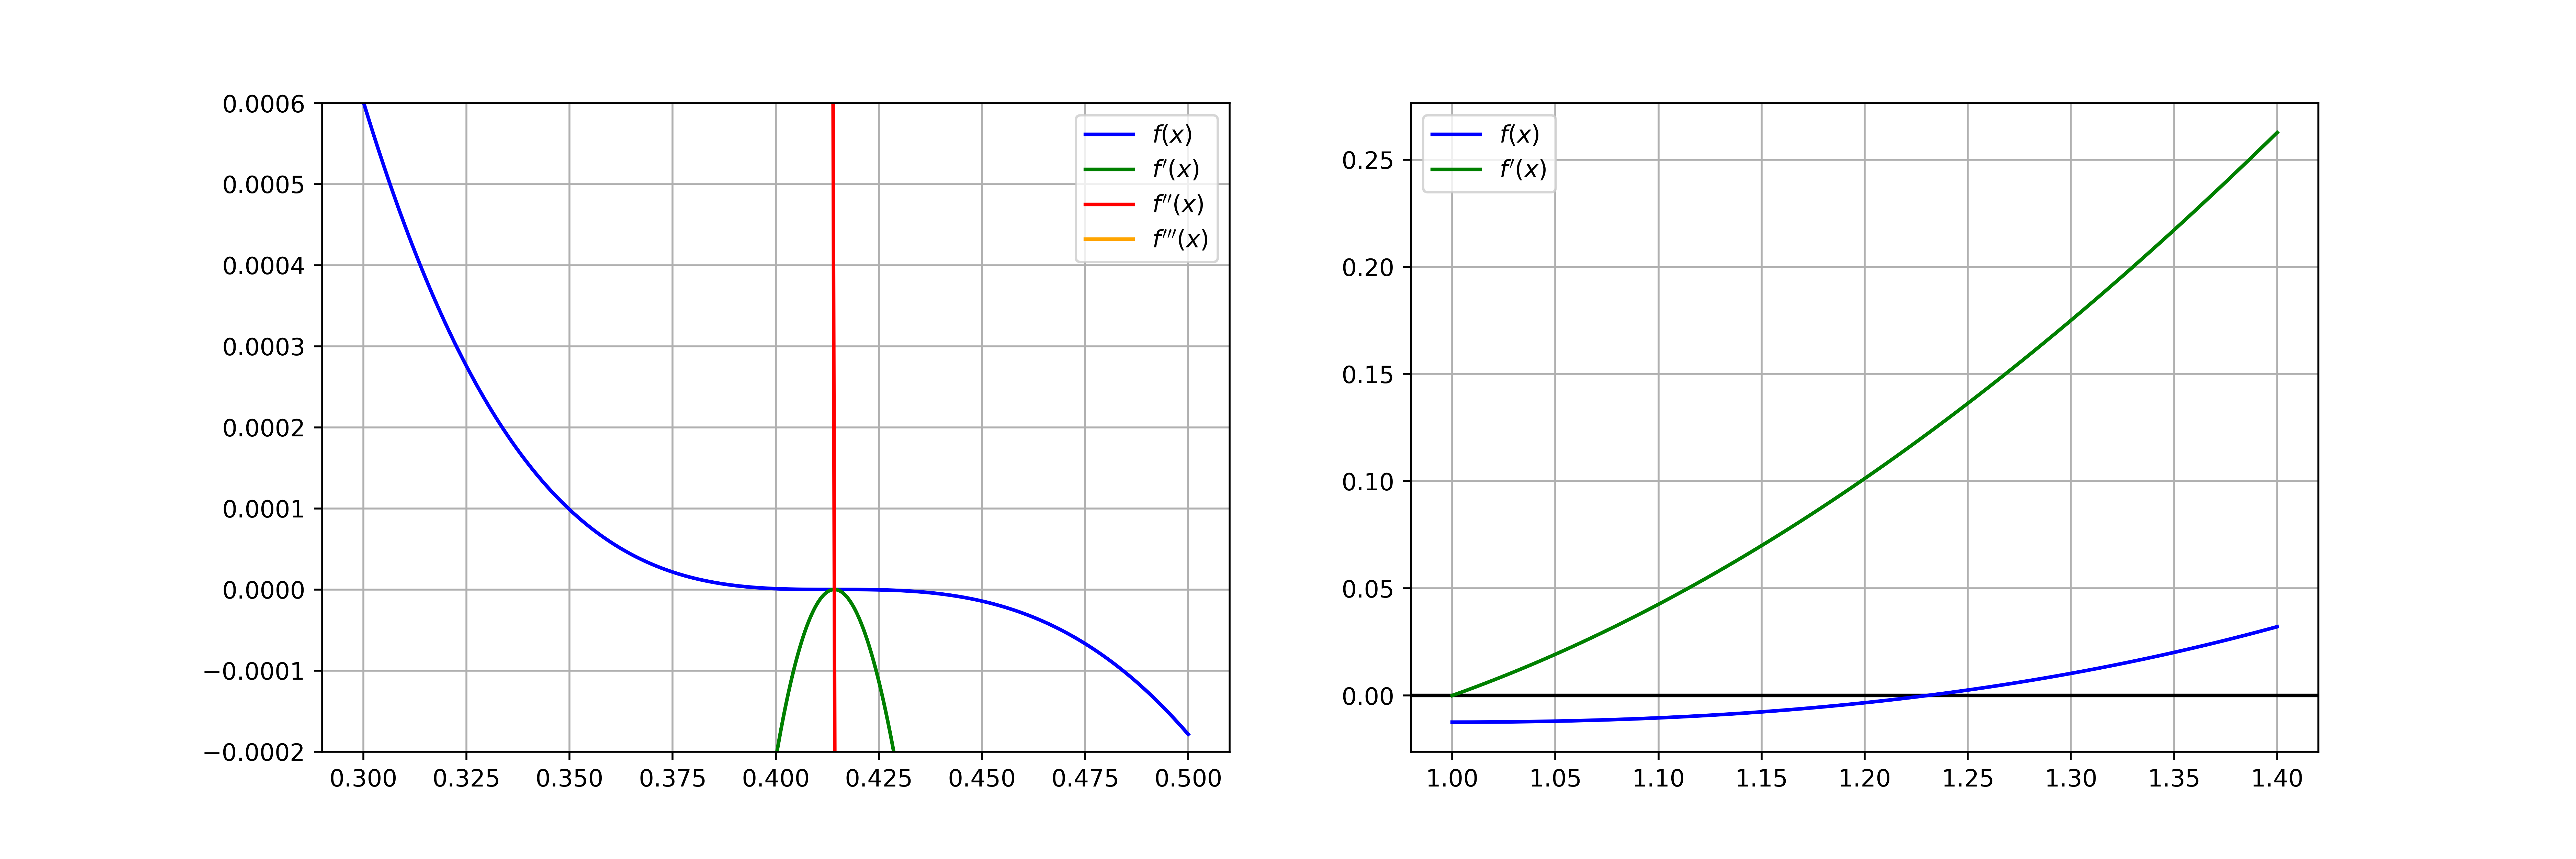
\includegraphics[width=18cm]{2.3_plot_d.png}

\vspace{2em}

В данной таблице представлены сравнительные решения $f(x) = 0$ различных методов для второго корня(Кратности 1):

\begin{tabular}{| c | c | c |}
	\hline
	Численный метод & Корень & Число итераций \\ \hline
	bisection & 1.230215553300 & 37 \\ \hline
	Newton method & 1.230215553299 & 6 \\ \hline
	Secant method & 1.230215553299 & 8 \\ \hline
	Steffensen method & 1.230215553299 & 6 \\ \hline
	Chord method & 1.230215553299 & 12 \\ \hline
	Neat Newton & 1.230215553299 & 13 \\ \hline
\end{tabular}

\vspace{2em}
Теперь приведем решение уравнения $f(x) = 0$ для корня кратности 3:

\begin{tabular}{| c | c | c |}
	\hline
	Численный метод & Корень & Число итераций \\ \hline
	bisection & 0.414202547132 & 35 \\ \hline
	Newton method & 0.414200921584 & 21 \\ \hline
	Secant method & 0.414203082835 & 23 \\ \hline
	Steffensen method & 0.413581653574 & 12 \\ \hline
	Chord method & 0.414198800334 & 8461 \\ \hline
	Neat Newton & 0.414198531775 & 24215 \\ \hline
\end{tabular}

\vspace{2em}

В следующей таблице решение уравнения $f''(x) = 0$ Тот же корень, но так как решаем уравнение со второй производной, то кратность - 1

\begin{tabular}{| c | c | c |}
	\hline
	Численный метод & Корень & Число итераций \\ \hline
	bisection & 0.414213562373 & 35 \\ \hline
	Newton method & 0.414213562373 & 5 \\ \hline
	Secant method & 0.414213562373 & 7 \\ \hline
	Steffensen method & 0.414213562373 & 6 \\ \hline
	Chord method & 0.414213562373 & 8 \\ \hline
	Neat Newton & 0.414213562373 & 7 \\ \hline
	Fixed point iter & 0.414213562373 & 7 \\ \hline
\end{tabular}

\vspace{2em}
Правильно ли я понимаю, что различия в ответе метода бисекции для уравнения $f(x) = 0$ и $f''(x) = 0$ уже в 5 знаке также обусловлены интервалом неопределенности корня? Тогда получается что на какой-то из своих итераций метод бисекции зашел не в тот отрезок из-за того, что посчитал произведение значений функции на краях отрезка $[a^{(k)}, b^{(k)}]$ равным нулю.

Истинным ответом, как мне кажется, следует считать решение уравнения $f''(x) = 0$ несмотря на трудоемкость поиска всех производных.

\end{document}